\section{Materials and methods}
\label{sec:method}

Our model, shown in Figure~\ref{fig:diagram}, takes in i.i.d. images, $\vec{X} = \set{\vec{X}\order{i}}^N_{i=1}$. For each image $\vec{x} = \vec{X}\order{i}$, it can the generate an HR image, $\tilde{\vec{x}}_{HR}$, from a downsampled LR version $\vec{x}_{LR}$, as close to the original image $\vec{x}_{HR}$.

For i.i.d. data like this, each pixel are assumed to follow a marginal joint probability distribution, which makes it possible to decompose the log-likelihood of each datapoint, $i$, in a sum $\log \dec{\vec{X}} = \sum^N_{i=1} \log \dec{\vec{X}\order{i}}$. 

\begin{figure*}
	\centering
	\usetikzlibrary{positioning}
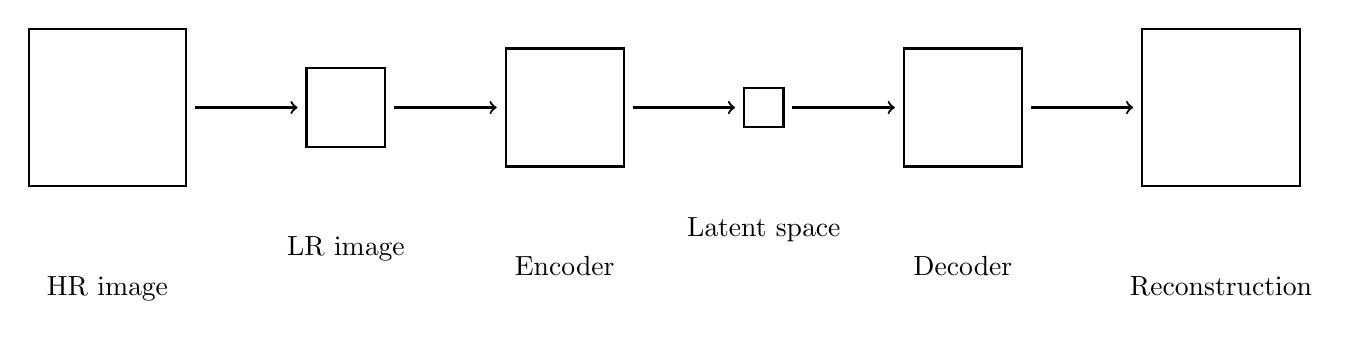
\begin{tikzpicture}[x = 1cm, y = 1cm, thick,
		image/.style={rectangle, draw, inner sep = 0pt, minimum size = 2 cm},
		network/.style={rectangle, draw, inner sep = 0pt, minimum size = 2 cm},
		arrow/.style={ ->, shorten <= 1 mm, shorten >= 1 mm}
	]
	
	\node[image, minimum size = 2 cm] (HR) at (0, 0) {};
	\node[below = of HR] {HR image};
	
	\node[image, minimum size = 1 cm, right = 1.5 cm of HR] (LR) {};
	\node[below = of LR] {LR image};
	
	\node[network, minimum size = 1.5 cm, right = 1.5 cm of LR] (encoder) {};
	\node[below = of encoder] {Encoder};
	
	\node[network, minimum size = 0.5 cm, right = 1.5 cm of encoder] (latent) {};
	\node[below = of latent] {Latent space};
	
	\node[network, minimum size = 1.5 cm, right = 1.5 cm of latent] (decoder) {};
	\node[below = of decoder] {Decoder};
	
	\node[image, minimum size = 2 cm, right = 1.5 cm of decoder] (reconstruction) {};
	\node[below = of reconstruction] {Reconstruction};
	
	\draw[arrow] (HR) -- (LR);
	\draw[arrow] (LR) -- (encoder);
	\draw[arrow] (encoder) -- (latent);
	\draw[arrow] (latent) -- (decoder);
	\draw[arrow] (decoder) -- (reconstruction);
	
\end{tikzpicture}

	\caption{Diagram of model. Originals $\vec{x}$ are binarised to $\vec{x}\idx{HR}$ and downsampled to $\vec{x}\idx{LR}$. Reconstructions, $\tilde{\vec{x}}\idx{HR}$, are the resulting output of the VAE.}
	\label{fig:diagram}
\end{figure*}

\subsection{Variational auto-encoder}
\label{sub:vae}

The VAE makes reconstructions from a underlying probabilistic data generating process inferring the same structure between similar digits. The similarity lies in the latent space, $\vec{z}$, which is the stochastic layer seen in the centre of the model in Figure~\ref{fig:diagram}. 

The input $\vec{x}_{LR}$ is mapped to the latent space through the encoder sampling from a normal distribution
$\vec{z} \sim \enc{\vec{z}|\vec{x}} = \mathcal{N}\parens{ \vec{z}|\vec{\mu}_\phi(\vec{x}),\vec{\sigma}^2_\phi(\vec{x})}$, where $\enc{\vec{z}|\vec{x}}$ is a variational approximation to the intractable true posterior $\dec{\vec{z}|\vec{x}}$.

Given the sampled $\vec{z}$, the decoder can generate a reconstruction $\tilde{\vec{x}}_{HR}$, where each pixel are assumed to be drawn from a Bernoulli distribution, $\vec{x} \sim \dec{\vec{x}|\vec{z}}=\mathcal{B}\parens{ \vec{x}|\vec{\mu}_\theta(\vec{z})}$, for binary data or from a normal distribution, $\vec{x} \sim \dec{\vec{x}|\vec{z}}=\mathcal{N}\parens{ \vec{x}|\vec{\mu}_\theta(\vec{z}),\vec{\sigma}^2_\theta(\vec{z})}$, for continuous data.

We want to find the distributions over a family of distributions that most likely produced the data. The model selection scheme is here variational Bayesian inference as Kingma et al \cite{Kingma2013} do using neural networks.  
 
The neural networks (NN) output the distribution parameters $\vec{\mu}_\phi(\vec{x})$ and $\vec{\sigma}^2_\phi(\vec{x})$ for the variational approximation $\enc{\vec{z}|\vec{x}}$ and $\vec{\mu}_\theta(\vec{z})$ for the conditional generative distribution $\dec{\vec{x}|\vec{z}}$.
% Instead of sampling from $\dec{\vec{x}|\vec{z}}$, we just draw $x=\vec{\mu}_\theta(\vec{z})$ as the most probable pixel values for the reconstruction.

To learn the variational parameters $\phi$ and the generative parameters $\theta$ (weights in the neural networks) jointly, we obtain a per-pixel training criterion from the variational lower bound $\mathcal{L}\parens{\vec{\theta},\vec{\phi};\vec{x}}$ derived from the mean-field approximation to the marginal log-likelihood:
\begin{equation}
	\log \dec{\vec{x}} = D\idx{KL}\parens{ \enc{\vec{z}|\vec{x}} \parallel \dec{\vec{z}|\vec{x}}} + \mathcal{L}\parens{\vec{\theta},\vec{\phi};\vec{x}} ,
\end{equation} 
where it is decomposed as for the EM-algorithm and variational inference \cite[\S10.2]{Bishop2006}. Here, the first term is the Kullback--Leibler divergence, which is a non-negative entropy measure of how much the approximated distribution $\enc{\vec{z}|\vec{x}}$ differs from the true posterior $\dec{\vec{z}|\vec{x}}$:
\begin{equation}
    D\idx{KL}\parens{ \enc{\vec{z}|\vec{x}} \parallel \dec{\vec{z}|\vec{x}}} = \int  \enc{\vec{z}|\vec{x}} \log \parens*{ \frac{\enc{\vec{z}|\vec{x}}}{\dec{\vec{x}|\vec{z}}} } \D{\vec{z}} .
\end{equation}

Since the KL divergence is non-negative, the second term (the ``free energy'') works as a variational lower bound and follows the inequality $\log \dec{\vec{x}} \ge \mathcal{L}\parens{\vec{\theta},\vec{\phi};\vec{x}}$, so maximising the lower bound with regards to the model parameters, we get $\mathcal{L}\parens{\vec{\theta},\vec{\phi};\vec{x}}\rightarrow \log \dec{\vec{x}}$, thereby pushing the KL divergence towards zero and bringing the approximated variational distribution closer to the true posterior.
The lower bound can be decomposed and rewritten as:
\begin{gather}
	\begin{split}
		\mathcal{L}\parens{\vec{\theta},\vec{\phi};\vec{x}} 
		& = \int \enc{\vec{z}|\vec{x}} \log \curlies*{ \frac{\dec{\vec{x},\vec{z}}}{\enc{\vec{z}|\vec{x}} } } \D{\vec{z}} \\
		& = \E_{\enc{\vec{z}|\vec{x}}} \brackets{- \log \enc{\vec{z}|\vec{x}} + \log \dec{\vec{x},\vec{z}} } 
		\\
		& = -D\idx{KL}\parens{ \enc{\vec{z}|\vec{x}} \parallel \dec{\vec{z}} }
        \\ & \hphantom{{}=}
        + \E_{\enc{\vec{z}|\vec{x}}} \brackets{\log \dec{\vec{x}|\vec{z}} } ,	
	\end{split}
\end{gather}
where the first term is another KL divergence acting as a regularisation term for $\vec{\phi}$ enforcing $\enc{\vec{z}|\vec{x}}$ to be similar to the prior $\dec{\vec{z}} = \mathcal{N}\parens{\vec{z}; \vec{0},\vec{I}}$. Leaving out this term would reduce the model to a normal auto-encoder with no restrictions on the distribution over $\vec{z}$ making it more likely to overfit on the training data.
% \begin{equation}
% 	-D\idx{KL}\parens{ \enc{\vec{z}|\vec{x}} \parallel \dec{\vec{z}} } = \frac{1}{2}\sum^J_{j+1}\parens{1 + \log \sigma_j ^2 - \mu_j^2 - \sigma_j^2}
% \end{equation}

The second term is the expected negative per-pixel reconstruction error, which has a differentiable Monte Carlo estimate:
\begin{equation}
	\E_{\enc{\vec{z}|\vec{x}}} \brackets{\log \dec{\vec{x}|\vec{z}} } \simeq \frac{1}{L}\sum^L_{l=1} \log \dec{\vec{x}|\vec{z}\order{l}}.
\end{equation}
where a reparameterisation trick is used for sampling $\vec{z}\order{l}= g_\phi (\vec{\epsilon}\order{l}, \vec{x})= \vec{\mu}_\phi(\vec{x}) + \vec{\sigma}_\phi(\vec{x}) \odot \vec{\epsilon}\order{l}$ with white noise sample $\vec{\epsilon}\order{l} \sim \mathcal{N}(\vec{0},\vec{I})$.\footnote{Here $\odot$ signifies element-wise
multiplication.}

Using this Monte Carlo estimate and a differentiable analytical evaluation of the KL term as in Kingma et al \cite{Kingma2013}, we obtain our final Stochastic Gradient Variational Bayes estimate, $\tilde{\mathcal{L}}\parens{\vec{\theta},\vec{\phi};\vec{X}\order{i}}$.

We use mini-batch gradient descent for obtaining the negative gradients $-\nabla_{\phi,\theta} \tilde{\mathcal{L}}^M\parens{\vec{\theta},\vec{\phi};\vec{X}\order{M}}$, which are used for updating the parameters $\phi$ and $\theta$ with the Adam method \cite{Kingma2014b} maximising the variational lower bound. 

% Differentiation of L
% Reparameretization trick
% Output parameters (mu and sigma)

% TODO: Add algorithm from Kingma13: Algorithm 1 Minibatch version of the Auto-Encoding VB (AEVB) algorithm.

\subsection{Experiments}
\label{sub:experiments}

We have trained our model on the MNIST dataset \cite{MNIST} of greyscale handwritten digits, combining the training set and validation set to get $60000$ images.  
To get a smaller number of configurations to reconstruct, we binarise the HR images before downsampling them by a factor of $d$ using a mean filter.
The binarisation is done by Bernoulli sampling for each pixel at every epoch, allowing for variations in the input data.

HR images was then reconstructed using our model for different values of latent size $N_{\vec{z}}$ and downsampling factor $d$ using a learning rate of $\num{e-3}$, which gave a good balance between computation time and steady non-oscillating learning curves indicating correct optimisation.
The encoder and decoder consists of two fully-connected neural networks with $200$ hidden neurones each using rectifiers as activation functions to obtain the features of a deep neural network without the high computation time.
The sampling size for the latent space was $L = 1$ and the mini-batch size was $M = 100$ as in Kingma et al \cite{Kingma2013}.
The reconstructions using our method are then compared to reconstructions upscaled using bicubic interpolation.
